\documentclass[11pt, oneside]{article}   	% use "amsart" instead of "article" for AMSLaTeX format
\usepackage{geometry}                		% See geometry.pdf to learn the layout options. There are lots.
\usepackage[parfill]{parskip}    			% Activate to begin paragraphs with an empty line rather than an indent
\usepackage{graphicx}						% Use pdf, png, jpg, or eps§ with pdflatex; use eps in DVI mode
											% TeX will automatically convert eps --> pdf in pdflatex
\usepackage{amssymb}
\usepackage{hyperref} 						% for \hyperfootnote
\usepackage{pifont}							% for \ding
\usepackage{url}							% for "plainurl" support in \bibliographystyle 
\usepackage{comment}
\usepackage{textcomp}						% for \langle and \rangle
\usepackage[dvipsnames]{xcolor}				% for text color definitions
\usepackage{listings}						% for json embedded listing

\colorlet{punct}{red!60!black}
\definecolor{background}{HTML}{EEEEEE}
\definecolor{delim}{RGB}{20,105,176}
\colorlet{numb}{magenta!60!black}
\lstdefinelanguage{json}{
    basicstyle=\footnotesize\ttfamily,
    numbers=left,
    numberstyle=\scriptsize,
    stepnumber=1,
    numbersep=8pt,
    showstringspaces=false,
    breaklines=true,
    frame=lines,
    backgroundcolor=\color{background},
    literate=
     *{0}{{{\color{numb}0}}}{1}
      {1}{{{\color{numb}1}}}{1}
      {2}{{{\color{numb}2}}}{1}
      {3}{{{\color{numb}3}}}{1}
      {4}{{{\color{numb}4}}}{1}
      {5}{{{\color{numb}5}}}{1}
      {6}{{{\color{numb}6}}}{1}
      {7}{{{\color{numb}7}}}{1}
      {8}{{{\color{numb}8}}}{1}
      {9}{{{\color{numb}9}}}{1}
      {:}{{{\color{punct}{:}}}}{1}
      {,}{{{\color{punct}{,}}}}{1}
      {\{}{{{\color{delim}{\{}}}}{1}
      {\}}{{{\color{delim}{\}}}}}{1}
      {[}{{{\color{delim}{[}}}}{1}
      {]}{{{\color{delim}{]}}}}{1},
}

% Make clickable footnote
\newcommand{\hyperfootnote}[1][]{\def\ArgI{{#1}}\hyperfootnoteRelay}
	% relay to new command to make extra optional command possible
\newcommand\hyperfootnoteRelay[2][]{\href{#1#2}{\ArgI}\footnote{\href{#1#2}{#2}}}
	% the first optional argument is now in \ArgI, the second is in #1
% Takes at most 3 parameters (see http://www.tex.ac.uk/FAQ-twooptarg.html for info on multiple optional parameters)
% If first parameter isn't given, it's value is '' (empty string in text before footnote reference)
% If second parameter isn't given, it's value is '' (string before visible URL, e.g. 'http://')
% Makes a clickable footnote (alternatively: \url{}) with optional reference in the text as well
% Use 1: \hyperfootnote{www.mywebsite.com}: creates a footnote consisting of a clickable URL
% Use 2: \hyperfootnote[My website]{www.mywebsite.com}: creates a clickable piece of text in the text ('My website') plus a footnote consisting of a clickable URL
% Note: requires the hyperref package.
% Note: use xspace package to add/absorb spaces when necessary (e.g. to avoid a space between the footnote number and a punctuation mark)
% Info on how to define a LaTeX command: https://www.sharelatex.com/learn/Commands

\geometry{letterpaper}                   	% ... or a4paper or a5paper or ... 
\usepackage{draftwatermark}
\SetWatermarkLightness{0.9}
\SetWatermarkText{DRAFT}					% you can use \today
\SetWatermarkScale{4}

\title{Age Protect}
\author{Paul Trevithick\footnote{The Mee Foundation}, Denise Tayloe\footnote{Privacy Vaults Online, Inc. dba PRIVO}, Alexander Yuhimenko\footnote{Swift Invention, Inc.}}
\date{May 29, 2023. Revised \today}							
\begin{document}
\maketitle
\begin{abstract}
	We present a new age verification approach with a unique combination of characteristics: (i) it is opt-in: a parent or guardian can choose to protect their minor children and adults can use it to prove they are of age (ii) the privacy and anonymity of all parties is respected (iii) it leaves the existing internet experience unchanged for those that don't opt-in. Age Protect is a technical specification that defines the interactions between three kinds of parties: online service providers, digital wallets, and age verification services (AVSes). Service providers can implement it to offer age-restricted content and services consistent with prevailing laws and regulations. People can use it by installing a compatible digital wallet and having a relationship with a compatible AVS. Using this wallet a person can convey AVS-attested age-related information to service providers which can use it to authorize access to content and services they offer on their apps, websites, or other online services. 
\end{abstract}

\section{Introduction}

Society agrees to supervise the places children inhabit, protect them from environments they should not encounter, and regulate the products they use. As a result, businesses are not permitted to sell tobacco, alcohol, pornography, handguns, certain kinds of fireworks, and other products and services to minors. However, none of this is true online. In the virtual world children are largely unprotected despite being exposed to a wide range of potential harms. 

Many approaches have been proposed and tried without much success. Existing laws have proven to be insufficient, and industry self-regulation has largely failed. Today there is a renewed global push to protect children's safety through stronger laws and regulations. Although some use other approaches\footnote{Such as requiring online services that are likely to be used by young people to default to the highest privacy setting possible for minors, as mandated by California's Age-Appropriate Design Code Act.}, many mandate age verification.\cite{Griswold2023}\cite{Jackson2023} However, privacy advocates and others have shown that many of the mechanisms for verifying age online weaken anonymity and privacy.\cite{Roth2023} 

Age Protect is a new age verification solution with a unique combination of characteristics: (i) it is opt-in; a parent or guardian can choose to protect their minor children and adults can use it to prove they are of age (ii) the privacy and anonymity of all parties is respected\footnote{This addresses the limitations of current age verification approaches\cite{Roth2023}} (iii) it leaves the existing internet experience completely unchanged.\footnote{The Age Protect approach is in contrast to age verification mandates. ``Age verification laws don’t just impact young people. It’s necessary to confirm the age of all website visitors, in order to keep out one select age group."\cite{Kelley2023}}

\section{Design Goals}

If Age Protect were widely adopted it would provide an age-aware experience for people that use apps, websites, and other online services. Its goals include:
\begin{itemize}
	\item \textbf{Opt-in}. The experience a person has at apps, websites and other online services remains unchanged unless Age Protect is enabled. If the person is an adult, they can turn it on themselves for their own benefit (e.g. to gain access to age-restricted services). If the person is a minor it can be turned on by their adult guardian on the minor's behalf. 
	\item \textbf{Protect minors}. Allow a guardian to enable Age Protect for a minor so that when the minor uses an online service the service receives an Age Protect signal. This signal indicates that this minor is capable of verifying their age on request (usually with one tap). Based on the age of the minor, the app/site can thereafter restrict access only to those services, features, activities, and marketing practices that are age-appropriate.
	\item \textbf{Age verify adults} so that they can prove (usually with one tap) that they are of sufficient age to access age-restricted apps and sites.
	\item \textbf{Respects the privacy} and anonymity of all participants.
	\item \textbf{Ease of use}. Provide a simple, intuitive user experience.
	\item \textbf{Reduce liability} for online service providers and protect their brand by helping them comply with laws and regulations such as \hyperfootnote[COPPA][https:]{ftc.gov/legal-library/browse/rules/childrens-online-privacy-protection-rule-coppa}, \hyperfootnote[GDPR][https://]{gdpr-info.eu/} (including the \hyperfootnote[UK Children's Code][https://]{ico.org.uk/for-organisations/uk-gdpr-guidance-and-resources/childrens-information/childrens-code-guidance-and-resources/}) and United States state age-appropriate design code regulations.
	\item \textbf{Cross-platform}. Age Protect can be implemented by service providers, digital wallets, and AVSes on a wide variety of internet connected platforms.
\end{itemize}
The following goals are out of scope\footnote{These goals could be achieved by implementations that add additional capabilities beyond those anticipated by this specification}:
\begin{itemize}
	\item \textbf{Give guardians control} to allow or block specific apps/sites a minor under their care can or cannot access or utilize, including specific services, features, or activities offered by that app/site.
	\item \textbf{Notify guardians} of privacy and safety notifications related to a minor's activities.
\end{itemize}

\section{Terminology}

Age Protect is a specification for the interactions between three kinds of entities: service providers, wallets, and Age Verification Services. 

A service provider offers apps, websites and other online services (and theoretically also by gaming consoles and Connected TVs)\footnote{This is an area for future research as to how the wallet-to-platform integration would best be achieved}. For the rest of this document we will refer to a service provider as a \emph{verifier} following the tradition used in the \hyperfootnote[Verifiable Credential(VC)][https://]{w3.org/TR/vc-data-model/} community, and defined below.

By \emph{digital wallet} we mean a specialized kind of software application running on a person's phone(s), tablet(s) and/or laptop(s) that stores and protects access to the wallet-holder's credentials and other kinds of personal data.\footnote{This specification could theoretically be extended in a straightforward way to also embrance ``Virtual'' or web-hosted wallets. We have not done so because these approaches require that the holder either trust an external administrative authority or must self-host. The former is problematic from a privacy/trust perspective, and the latter from a cost/competence perspective}. For the balance of this document we use term wallet as a synonym for the term \emph{repository} used in the VC community and defined below.

By \emph{Age Verification Services (AVSes)} we mean a third-party online service and/or mobile app that provides age and identity verification services. For the balance of this document we refer to the AVS as an \emph{issuer} following the tradition used in the VC community and defined below.

\begin{itemize}
	\item \textbf{holder}: A role an entity might perform by possessing one or more verifiable credentials and generating presentations from them. A holder is usually, but not always, a subject of the verifiable credentials they are holding. Holders store their credentials in credential repositories.
	\item \textbf{issuer}: A role an entity can perform by asserting claims about one or more subjects, creating a verifiable credential from these claims, and transmitting the verifiable credential to a holder.
	\item \textbf{presentation}: Data derived from one or more verifiable credentials, issued by one or more issuers, that is shared with a specific verifier.
	\item \textbf{repository}: A program, such as a storage vault or personal verifiable credential wallet, that stores and protects access to holders' verifiable credentials.
	\item \textbf{subject}: A thing about which claims are made. 
	\item \textbf{verifiable presentation}: A verifiable presentation is a tamper-evident presentation encoded in such a way that authorship of the data can be trusted after a process of cryptographic verification. Certain types of verifiable presentations might contain data that is synthesized from, but do not contain, the original verifiable credentials (for example, zero-knowledge proofs).
	\item \textbf{verifier}: A role an entity performs by receiving one or more verifiable credentials, optionally inside a verifiable presentation for processing. 
\end{itemize}	

\section{Usage Scenarios} 

For simplicity in this section we describe only scenarios involving websites rather than mobile apps, although the principles are the same.

For Age Protect to work a person must have a compatible wallet containing an \emph{Age Verification Record (AVR)} document issued by a compatible AVS. After they have achieved this, their experience at Age Protect-compatible apps/sites (verifiers) will change. If the app/site needs to verify their age the verifier will display a \emph{Verify Age} button that when tapped initiates a \hyperfootnote[\emph{verifiable presentation request}][https://]{w3c-ccg.github.io/vp-request-spec/} to learn the holder's age. The wallet responds to this request, and based on the holder's age the holder will gain or be denied access to one or more kinds of content and services provided by the verifier. 

Age Protect can be used by both minors and adults, and we will describe usage scenarios for both. Although Age Protect supports scenarios where a single guardian protects multiple minors, for simplicity we will describe only the single-minor use case. It can also support multiple people sharing the same tablet or laptop by relying on the wallet's ability to do the same. The wallet would need to identify the holder uniquely even if biometric identification was not supported by the hardware by requiring an additional credential such as a PIN code.

In this document we refer to a \emph{Verify Age button}. This is a button on the service provider (verifier) app/site initiate a verifiable presentation request to the wallet holder's wallet in order to obtain the holder's age as claimed by the issuer.

\subsection{Adult verifies age on a website}

The simplest scenario involving an adult playing the role of both subject and holder. They first acquire an \emph{Age Verification Record(AVR)} from an issuer, store it in their wallet, and then go to an age-restricted website of a service provider (verifier) where they are asked to prove their age. The \hyperfootnote[digital wallet][https://]{openwallet.foundation/} holds the AVR from which a presentation is computed and shared with the verifier. An AVR is a \hyperfootnote[VC][https://]{w3.org/TR/vc-data-model/} which contains a claim whose value is the birthdate of the adult as asserted by the AVS. The presentation data (including the age claim) can be verified cryptographically by the verifier as being issued by an issuer that they trust.

This scenario is shown in Figure \ref{fig:adult}. We describe each numbered step in the flow: 

\begin{enumerate}
	\item The adult goes to an age verification service (issuer), logs in, and begins identity verification using whatever methods are supported by the issuer. 
	\item After the adult has completed identity verification, the issuer issues them an AVR. This AVR is transmitted to the adult's wallet.
	\item The adult visits the service provider's (verifier's) website. In the HTTP header the wallet includes an Age Protect header (defined using \hyperfootnote[ProviderDiscovery][https://]{providerdiscovery.org}) which is detected by the verifier. 
	\item Whenever the verifier needs to verify the age of the person they display the Verify Age button.
	\item The adult (holder) taps the Verify Age button, which opens their wallet. The wallet retrieves the necessary AVR, and asks the adult to consent to share a presentation of it with the website as proof of their age. 
\end{enumerate}

Additional details are provided in the sequence diagram in Figure \ref{fig:adult-seq}. 

\begin{figure}
	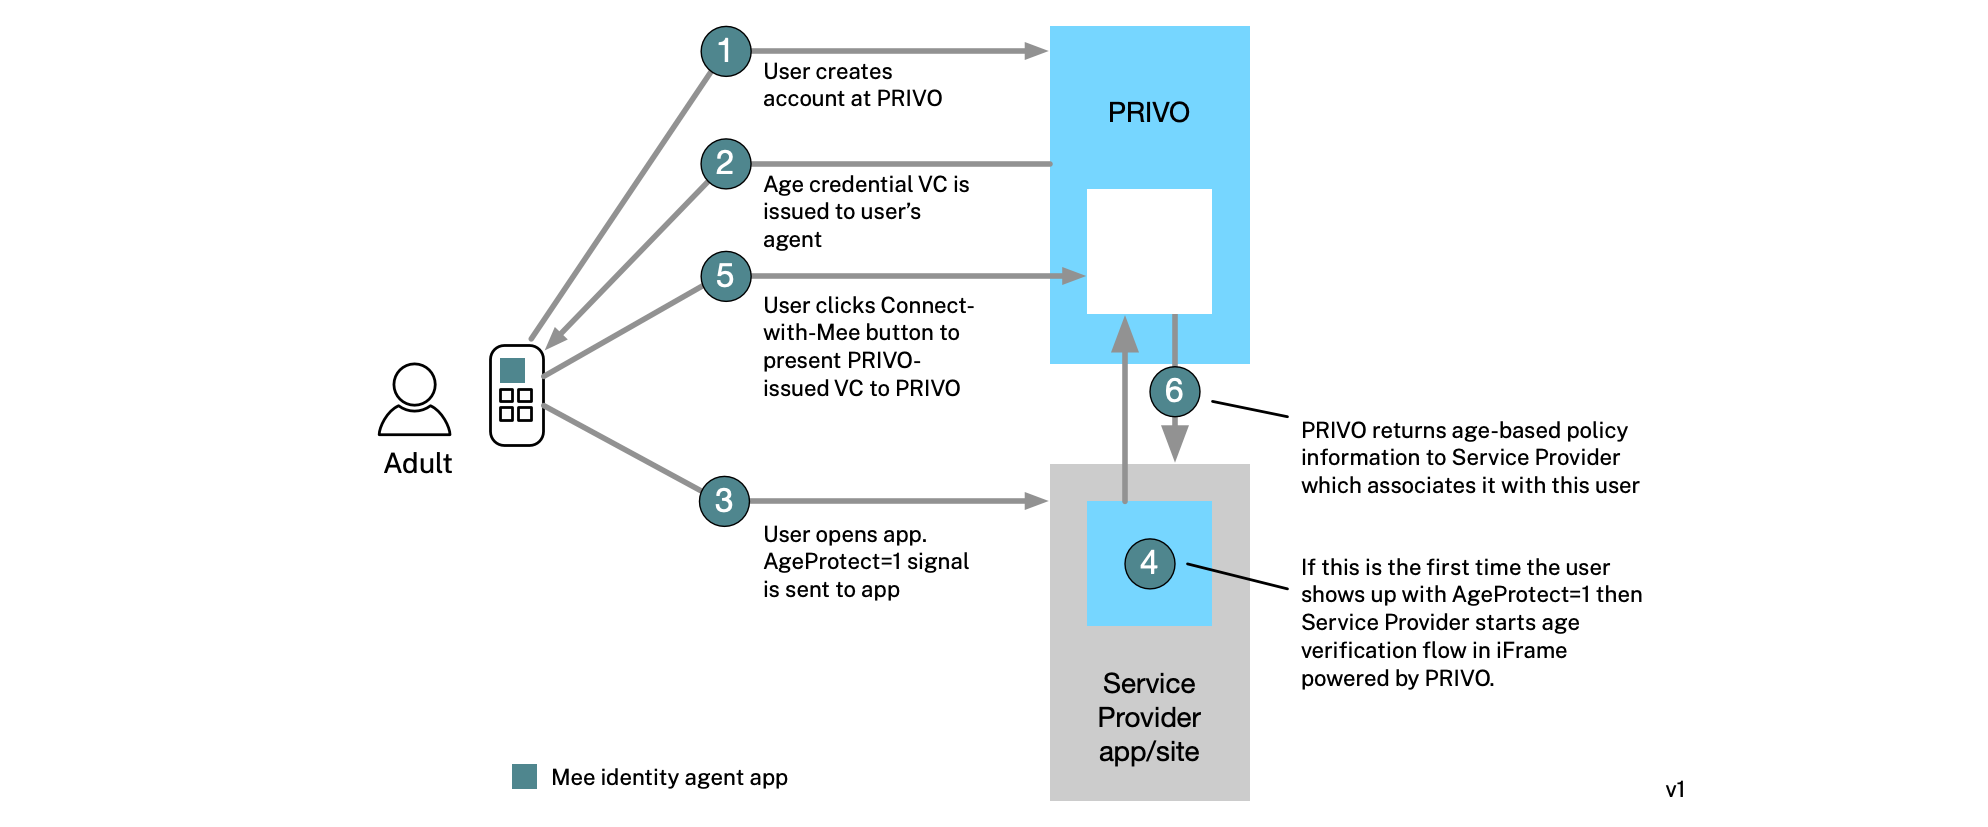
\includegraphics[width=\textwidth]{./images/adult.png}
	\caption{Adult gets AVR and visits a verifier's website}
	\label{fig:adult}
\end{figure}

\begin{figure}
	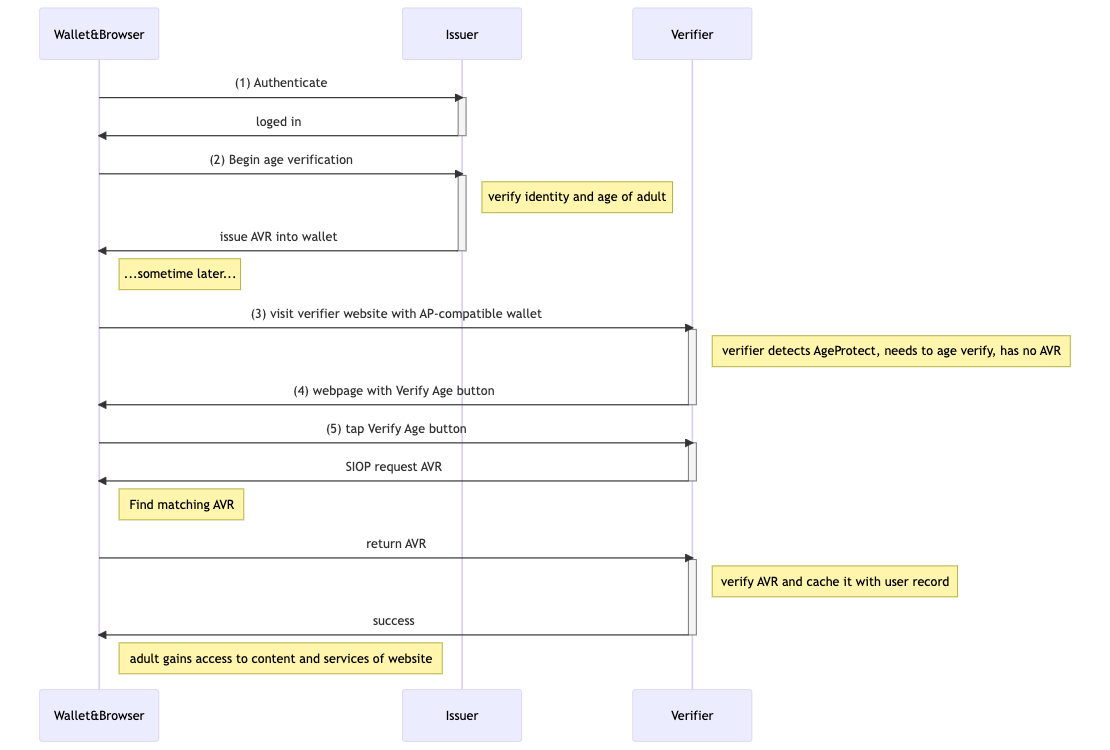
\includegraphics[width=\textwidth]{./images/adult-sequence.png}
	\caption{Adult gets AVR and visits a verifier's website}
	\label{fig:adult-seq}
\end{figure}
\begin{comment}
MERMAID
sequenceDiagram
    participant Wallet&Browser
    participant Issuer
    participant Verifier
    Wallet&Browser->>+Issuer: (1) Authenticate
    Wallet&Browser->>+Issuer: (2) Begin age verification
    Note right of Issuer: verify identity and age of adult
    Issuer->>-Wallet&Browser: issue AVR into adult's wallet
    Note right of Wallet&Browser: ...sometime later...
    Wallet&Browser->>+Verifier: (3) visit verifier website with AP-compatible wallet
    Note right of Verifier: verifier detects AgeProtect, needs to age verify, has no AVR
    Verifier->>-Wallet&Browser: (4) webpage with Verify Age button
    Wallet&Browser->>+Verifier: (5) tap Verify Age button
    Verifier->>-Wallet&Browser: SIOP request AVR
    Note right of Wallet&Browser: Find matching AVR
    Wallet&Browser->>Verifier: return AVR
    Note right of Verifier: verify AVR and cache it with user record
    Note right of Verifier: adult gains access to content and services of website

\end{comment}

\subsection{Minor verifies age at a website}

In this scenario we show how a minor can verify their age at a verifier leveraging the fact that they were previously registered by a guardian at an issuer and issued with an AVR. In this scenario, the minor is acting in the holder role and can take this AVR to any website without being tracked by the guardian or any other entity. 

The guardian registers a minor (e.g. child) at an AVS issuer, shares a link (or QR code) with this minor, and the minor then visits a website that has implemented Age Protect. This flow, shown in Figure \ref{fig:guardian+minor}, has the following steps:
\begin{enumerate}
	\item The guardian goes to an AVS (issuer) website, logs in, and begins identity verification on themselves (using whatever methods are supported by the issuer). They then register the minor, a process that includes specifying the minor's birthdate.
	\item A link (and QR code) is generated for the minor and made available to the guardian.
	\item The guardian shares this link (or QR code) with the minor.
	\item The minor scans the QR code (or taps the URL) which brings them to the issuer's website. An AVR is transmitted to their wallet.
	\item The minor goes to the verifier's website. The HTTP header contains the Age Protect header (defined using \hyperfootnote[ProviderDiscovery][https://]{providerdiscovery.org}) which is observed by the verifier.
	\item When the verifier needs to verify the age of their visitor it displays a page with a Verify Age button prompting the minor to tap it and thereby request the minor's age.
	\item The minor taps the Verify Age button. Doing so begins a presentation request to the minor's wallet. The wallet response with a verifiable presentation containing the requested information.
\end{enumerate}

\begin{figure}
	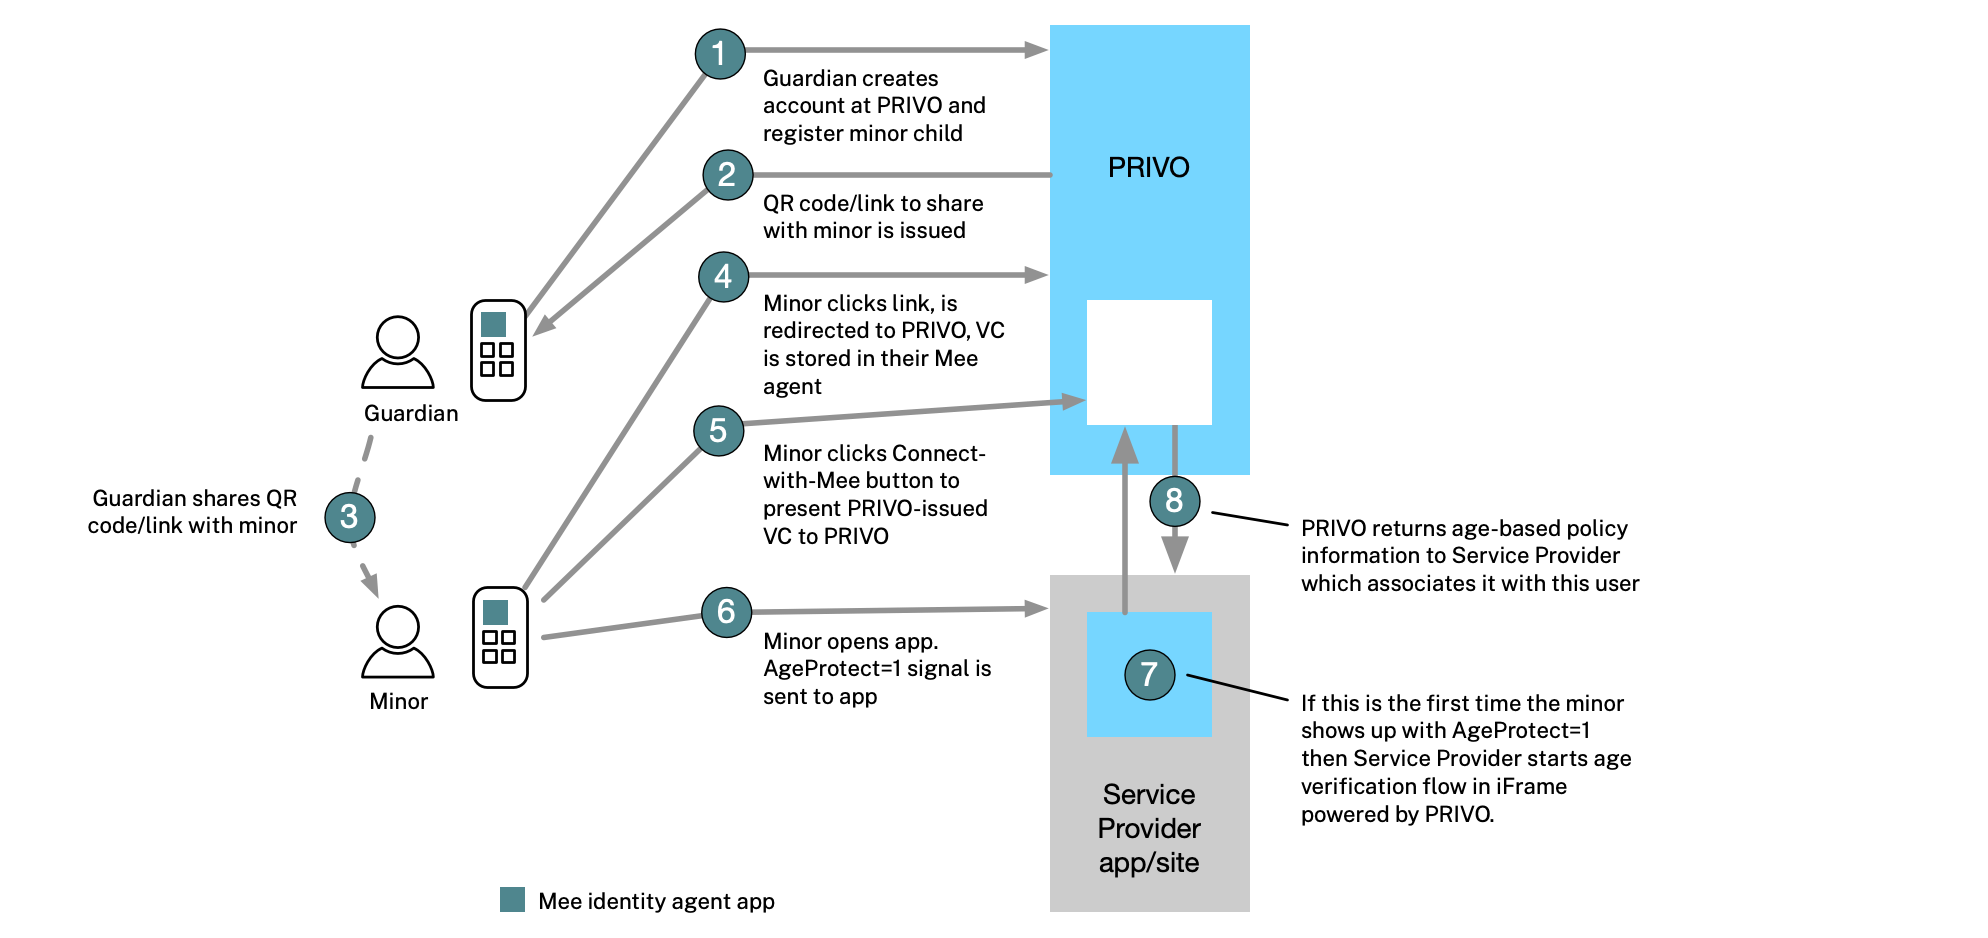
\includegraphics[width=\textwidth]{./images/guardian+minor.png}
	\caption{Minor with guardian flow}
	\label{fig:guardian+minor}
\end{figure}

\begin{comment}
\subsection{Consent: allowing/blocking access to a website by a minor}

In the previous scenario the minor was free to use any Age Protect-compatible website so long as the information in their AVR met the age criteria of the website. In this scenario we go further and show how the guardian can control the minor's access to specific websites and even specific kinds of services within a website (e.g. the ability to chat with others, upload images, etc.).

Here's a rough sketch of how this works. Every time the minor wishes to access a new website they must first possess (i.e. have stored in their wallet) an authorization token for it. For example if the minor wants to visit Facebook.com they must first have a token for Facebook.com. This token is issued by an interaction between the AVS and the guardian. 

Here's how the flow works the first time the minor attempts to go to Facebook.com: 
\begin{enumerate}
	\item Minor attempts to visit Facebook.com
	\item Their wallet's browser extension attempts to fetch from their wallet an authorization token (issued by an AVS) that specifies that the minor is permitted to visit Facebook.com. In this scenario no such token exists.
	\item The minor's wallet sends a request for authorization to the guardian's wallet (leveraging the digital connection between the guardian's wallet and the minor's wallet)
	\item The guardian's wallet invokes the AVS app/site. This app/site provides a UI that enables the guardian to manage an ``allowed list'' and a ``blocked list'' of SPs. Using this UI the guardian modifies these lists to allow or block access to Facebook.com. If access is allowed it generates a token encoding this capability. 
	\item The AVS issues the token to the guardian by adding it into a storage area within the guardian's wallet that is associated with the guardian's relationship with the AVS.
	\item The guardian's wallet sends this token to the minor's wallet (leveraging the digital connection between the guardian's wallet and the minor's wallet, [and specifically replication of the storage area in the guardian's wallet])
	\item The minor's wallet verifies this token and communicates with the browser extension to allow the browser to proceed to Facebook.com
\end{enumerate}
\end{comment}

\subsection{Minor uninstalls their wallet}

A minor can attempt to disable Age Protect by uninstalling the wallet from their devices. However, the wallet, just before the uninstallation process completes, sends a signal to the AVS. The AVS can in turn notify the minor's guardian that the minor has uninstalled their wallet.

\section{Technical specifications}

\subsection{Age Protect Signaling}
 
An Age Protect-compatible wallet relies on a browser extension that implements the \hyperfootnote[Provider Discovery][https://]{providerdiscovery.org} specification. The browser extension includes the \emph{Sec-PD} HTTP header field with a value of \emph{AgeProtectv1}:
\begin{lstlisting}[language=json,firstnumber=1]
	Sec-PD: type=AgeProtectv1
\end{lstlisting}

Optionally, if the person already has a relationship with a specific age verification provider, e.g. PRIVO.com, they could configure their browser extension to send an enriched HTTP header field:
\begin{lstlisting}[language=json,firstnumber=1]
	Sec-PD: type=AgeProtectv1; cfg="https://privo.com/age-protect.pcf"
\end{lstlisting}
\subsection{Verify Age button}

This subsection will describe how the Verify Age button is implemented. 

\subsection{Age Verification Record}

An AVR is a Verifiable Credential (VC)\hyperfootnote[Verifiable Credential][https://]{w3.org/TR/vc-data-model/} JSON document. 

\textbf{@Context property}

The \emph{@Context} property must include at least these two values:
\begin{itemize}
	\item ``https://www.w3.org/2018/credentials/v1''
	\item ``https://schema.mee.foundation/age-protect/v1''
\end{itemize}

\textbf{id property}

The \emph{id} property must uniquely identify this type of AVR document. 
	
\textbf{type property}

The \hyperfootnote[\emph{type}][https://]{w3.org/TR/vc-data-model/\#types} property must be present and contain these two values:
\begin{itemize}
	\item ``VerifiableCredential''
	\item ``AgeProtectAVR''
\end{itemize}

\textbf{issuer property}

The \hyperfootnote[\emph{issuer}][https://]{w3.org/TR/vc-data-model/\#issuer} property must be present.

\textbf{credentialSubject property}

The \hyperfootnote[\emph{credentialSubject}][https://]{w3.org/TR/vc-data-model/\#credential-subject} property must be present. It must include the following sub-properties:
\begin{itemize}
	\item \emph{birthdate} - the subject's (i.e., holder's) birthdate
	\item \emph{ageOrOver} - the age of the subject at AVR issuance
	\item \emph{jurisdiction} - the jurisdiction where the subject lives. 
	\begin{itemize}
		\item \emph{countryCode} - in \hyperfootnote[ISO 3166-1]["https://"]{https://en.wikipedia.org/wiki/ISO\_3166-1} format
		\item \emph{subdivisionCode} - in \hyperfootnote[ISO 3166-2][https://]{https://en.wikipedia.org/wiki/ISO\_3166-2} format
	\end{itemize}
\end{itemize}

\textbf{credential-subject property}

The \emph{credential-subject} property may include the following optional sub-properties:
\begin{itemize}
	\item \emph{ageUnder13} - boolean
	\item \emph{age13OrOver} - boolean
	\item \emph{ageUnder14} - boolean
	\item \emph{ageUnder15} - boolean
	\item \emph{ageUnder16} - boolean
	\item \emph{ageUnder17} - boolean
	\item \emph{ageUnder18} - boolean
	\item \emph{age18OrOver} - boolean
	\item \emph{age20OrOver} - boolean
	\item \emph{ageUnder21} - boolean
	\item \emph{age21OrOver} - boolean
	\item \emph{age25OrOver} - boolean
	\item \emph{age55OrOver} - boolean
	\item \emph{age60OrOver} - boolean
	\item \emph{age65OrOver} - boolean
	\item \emph{id} - a subject identifier defined by the issuer
	\item \emph{ageVerificationMethod} - oneOf (``AgeEstimation'', ``GovernmentID'', ``ThirdParty'')
\end{itemize}

\textbf{credentialStatus property}

The \hyperfootnote[\emph{credentialStatus}][https://]{w3.org/TR/vc-data-model/\#status} property must be present.

\textbf{ageAssertionProvider property}

The \emph{ageAssertionProvider} property must be present. Allowed values are oneOf (``Guardian'', ``Parent'', ``Self'')

\textbf{assuranceLevel property}

The \emph{assuranceLevel} property must be present. Its values are defined by \hyperfootnote[fhir.org][https://]{https://build.fhir.org/ig/HL7/fhir-identity-matching-ig/guidance-on-identity-assurance.html} which we summarize as oneOf (``IAL1'', ``IAL1.2'', ``IAL1.5'', ``IAL1.6'', ``IAL1.8'', ``IAL2'')

\textbf{issuanceDate property}

The \hyperfootnote[\emph{issuanceDate}][https://]{w3.org/TR/vc-data-model/\#issuanceDate} property must be present.

\textbf{expirationDate property}

The \hyperfootnote[\emph{expirationDate}][https://]{w3.org/TR/vc-data-model/\#expirationDate} property must be present.

\textbf{nonTransferable property}

The \hyperfootnote[\emph{nonTransferable}][https://]{w3.org/TR/vc-data-model/\#nontransferable-property} property must have a value of true to prevent the VC from being allowed to be transferred to another wallet.

\textbf{proof property}

The \hyperfootnote[\emph{proof}][https://]{w3.org/TR/vc-data-model/\#proofs-signatures} property must be present to allow the verifier to validate the presentation data derived from the AVR.

Here is a sample AVR document:

\begin{lstlisting}[language=json,firstnumber=1]
{
	"@context": [
		"https://www.w3.org/2018/credentials/v1",
		"https://schema.mee.foundation/age-protect/v1"
	],
	"id": "https://age.privo.com/credentials/2015",
	"type": [
		"VerifiableCredential",
		"AgeProtectAVR"
	],

	"issuer": {
		"id": "https://vc.privo.com/issuer",
		"name": "PRIVO"
	},

	"credentialSubject": {
		"id": "https://vc.privo.com/age/ebfeb1f712ebc6f1c276e12ec21",
		"birthdate": "2010-09-15",
		"ageOrOver": 12,
		"ageUnder13" : true,
		"age21OrOver: false,
		"jurisdiction": {
			"countryCode" : "US",
			"subdivisionCode": "VA"
		},
		"ageVerificationMethod": "AgeEstimation"
	},
	"ageAssertionProvider" : "parent",
	"assuranceLevel" : "L1.5",
	"issuanceDate": "2023-07-14T00:00:00Z",
	"expirationDate": "2024-09-15T00:00:00Z",
	"nonTransferable": true,
	"proof": {
		"created": "2023-07-15T13:13:39Z",
		"type": "CLSignature2019",
		"issuerData": "<...>",
		"attributes": "<...>",
		"signature": "<...>",
		"signatureCorrectnessProof": "<...>"
	}
}
\end{lstlisting}

\subsection{A few notes on AVR issuance}

To maximize privacy, the wallet relies on \hyperfootnote[\emph{selective disclosure}][https://]{w3.org/TR/vc-imp-guide/\#selective-disclosure}, thus the issuer must encrypt the AVR using algorithms that are compatible with selective disclosure.

To enhance the privacy of the person (holder), we may recommend that the AVR expiration is at most six months from issuance. 

\subsection{A few notes on AVR presentation by the wallet}

To maximize privacy we leverage \hyperfootnote[selective disclosure][https://]{w3.org/TR/vc-imp-guide/\#selective-disclosure}. This means that only the minimal set of claims requested by the verifier will be presented by the wallet. For example if only age is required, then only age will be presented, but not birthdate. We rely on verifiers being diligent to only request the minimal set of claims necessary. Along the same lines the \emph{jurisdiction} and/or \emph{ageVerificationMethod} are only presented to the verifier if requested. 

The expiration date is never presented to the verifier.

For performance reasons, we may recommend that the wallet compute a persistent unique to a verifier identifier for the wallet holder that expires after a certain amount of time (perhaps 30 days). This would enable caching by the verifier of the AVR record for this same period of time. This idea creates the possibility that the person is up to this amount of time older than the age claimed in the AVR. 

\section{Implementation}

To be written. This section will describe a prototype implementation of Age Protect being developed by \hyperfootnote[PRIVO][https://]{privo.com}, an AVS provider, \hyperfootnote[The Mee Foundation][https://]{mee.foundation}, a digital wallet provider, and \hyperfootnote[Swift Invention.][https://]{swiftinvention.com}, a software development firm.

\section{Conclusions and further work}
We have described the design of a new, opt-in, privacy-preserving age verification approach. This paper will be continuously updated as progress continues on the specifications and a prototype implementation.

\bibliography{../library}
\bibliographystyle{plainurl}
\end{document}  